\documentclass[11pt,a4paper]{article}

\usepackage[utf8]{inputenc}
\usepackage[T1]{fontenc}
\usepackage{lmodern}
\usepackage[french]{babel}
\usepackage[margin=2.2cm]{geometry}
\usepackage{amsmath,amssymb}
\usepackage{booktabs,tabularx,array,multirow}
\usepackage{graphicx}
\usepackage[table]{xcolor}
\usepackage{tikz}
\usetikzlibrary{arrows.meta,positioning}
\usepackage{tcolorbox}
\tcbuselibrary{skins,breakable}
\usepackage{enumitem}
\usepackage{caption}
\usepackage{float}
\usepackage{fancyhdr}
\usepackage{listings}
\usepackage[hidelinks]{hyperref}

\graphicspath{{figures_colab/}}

\definecolor{bleu}{HTML}{1F4E79}
\definecolor{bleuclair}{HTML}{E8F0F8}
\definecolor{vert}{HTML}{2E7D32}
\definecolor{vertclair}{HTML}{E8F5E9}
\definecolor{orange}{HTML}{E65100}
\definecolor{orangeclair}{HTML}{FFF3E0}
\definecolor{violet}{HTML}{5E35B1}
\definecolor{violetclair}{HTML}{EDE7F6}
\definecolor{gris}{HTML}{F5F5F5}

\newtcolorbox{resume}[1][]{colback=bleuclair,colframe=bleu,fonttitle=\bfseries,title=#1,breakable}
\newtcolorbox{constat}[1][]{colback=vertclair,colframe=vert,fonttitle=\bfseries,title=#1,breakable}
\newtcolorbox{attention}[1][]{colback=orangeclair,colframe=orange,fonttitle=\bfseries,title=#1,breakable}
\newtcolorbox{oral}[1][]{colback=violetclair,colframe=violet,fonttitle=\bfseries,title=#1,breakable}

\lstset{basicstyle=\ttfamily\small,backgroundcolor=\color{gris},frame=single,rulecolor=\color{gray!40},
        columns=fullflexible,keepspaces=true,breaklines=true,showstringspaces=false,
        literate={é}{{\'e}}1 {è}{{\`e}}1 {à}{{\`a}}1 {ô}{{\^o}}1 {ê}{{\^e}}1}

\setlist{itemsep=2pt,topsep=4pt}
\renewcommand{\arraystretch}{1.2}

\pagestyle{fancy}
\fancyhf{}
\lhead{\small Projet CAMELYON17 — le notebook Colab expliqué}
\rhead{\small \thepage}
\setlength{\headheight}{14pt}

\title{\vspace{-1.2cm}\textbf{\color{bleu}Projet CAMELYON17}\\[4pt]
\large Détecter le cancer sur des images de ganglions avec un CNN\\[2pt]
\normalsize Tout ce que contient le notebook Colab, expliqué pas à pas\\
\normalsize (support pour le suivi de 30 minutes avec la professeure)}
\author{L'équipe}
\date{12 novembre 2026}

\begin{document}
\maketitle
\thispagestyle{fancy}

\begin{resume}[À lire en premier : le message à faire passer demain]
\textit{« On a commencé par analyser les données, on a construit un premier petit modèle (un CNN classique)
qui sert de base commune, et maintenant chacun de l'équipe teste son propre modèle dans son coin, avec les
mêmes données, le même découpage et les mêmes métriques, pour qu'on puisse comparer honnêtement. »}

\medskip
\textbf{En chiffres (notre exécution du notebook)} :
\begin{itemize}
  \item 19\,254 images (\emph{patchs}) de 96 × 96 pixels, issues de 50 lames, 43 patientes, 5 hôpitaux ;
  \item un CNN de 389\,410 paramètres, appris de zéro, entraîné 300 époques sur 3 hôpitaux ;
  \item excellent sur les hôpitaux connus (AUC 0,999), moins bon sur des hôpitaux jamais vus
        (AUC 0,947 et 0,907) ;
  \item \textbf{le vrai problème} : au seuil réglé sur les hôpitaux connus, le modèle ne détecte plus que
        \textbf{35 \%} des tumeurs de l'hôpital 2. C'est le \emph{changement de domaine} : la couleur des
        lames change d'un hôpital à l'autre et le modèle se fait piéger.
\end{itemize}
\end{resume}

\noindent\textbf{Comment utiliser ce document.} Il suit les 9 parties du notebook Colab, dans le même ordre.
Pour chaque partie : \emph{ce qu'on fait}, \emph{pourquoi}, \emph{ce qu'on obtient}. Les encadrés
\colorbox{violetclair}{violets} donnent les questions que la professeure risque de poser, avec la réponse.
À la fin : un glossaire (section~\ref{sec:glossaire}) et \textbf{la liste des questions à lui poser}
(section~\ref{sec:questions}).

\tableofcontents
\newpage

%=====================================================================
\section{Le problème médical et l'objectif}
%=====================================================================

\subsection{Le contexte}
Dans le cancer du sein, le chirurgien retire les \textbf{ganglions lymphatiques} de l'aisselle pour savoir si
le cancer s'y est propagé. Une tumeur trouvée dans un ganglion s'appelle une \textbf{métastase}. C'est
décisif pour le traitement : une métastase change le \emph{stade} de la maladie, donc la chimiothérapie,
la radiothérapie, etc.

Chaque ganglion est coupé en tranches très fines, coloré, puis numérisé au microscope. On obtient une
\textbf{lame entière} (en anglais \emph{whole slide image}, WSI) : une image gigantesque d'environ
100\,000 × 200\,000 pixels, qui pèse 1 à 3 Go.

\paragraph{La coloration H\&E.} Sans colorant, le tissu est transparent. On utilise deux colorants :
\begin{itemize}
  \item l'\textbf{hématoxyline} colore les \emph{noyaux} des cellules en violet / bleu ;
  \item l'\textbf{éosine} colore le \emph{cytoplasme} et les fibres en rose.
\end{itemize}
Chaque hôpital a sa propre recette de coloration et son propre scanner : les images n'ont pas toutes la même
couleur. Ce détail est au cœur de tout le projet.

\subsection{Pourquoi automatiser ?}
Un pathologiste (médecin spécialiste des tissus) parcourt chaque lame à la recherche de cellules tumorales.
C'est long, fatigant, et les \textbf{petites métastases peuvent être ratées}. Un modèle peut servir
d'assistant : il signale les zones suspectes, le médecin vérifie.

\subsection{L'objectif de cette première étape}
Apprendre à un modèle à répondre, pour chaque petit carré d'image de 96 × 96 pixels (un \textbf{patch}) :
\begin{center}
\textit{« Ce patch contient-il du tissu tumoral (1) ou non (0) ? »}
\end{center}
C'est une \textbf{classification binaire d'images} (deux classes possibles).
Plus tard (étape 2, hors du notebook), on assemble les prédictions de tous les patchs d'une lame pour former
une \emph{carte de chaleur}, puis on en déduit le \emph{stade pN} de la patiente.

\begin{attention}[La priorité qui guide tous nos choix]
Une \textbf{métastase ratée} (faux négatif) est bien plus grave qu'une \textbf{fausse alerte} (faux
positif) : dans le premier cas, la patiente risque de ne pas recevoir le traitement dont elle a besoin ;
dans le second, le médecin regarde une zone de plus pour rien. On va donc surveiller en priorité la
\textbf{sensibilité} (la part des tumeurs détectées), et pas seulement la « précision globale ».
\end{attention}

%=====================================================================
\section{Les données}
%=====================================================================

\subsection{Lesquelles ?}
On utilise \textbf{Camelyon17-WILDS} (Koh et al., 2021), une version « prête à l'emploi » du challenge
international \textbf{CAMELYON17} (Bándi et al., 2019).

\begin{table}[H]
\centering
\begin{tabularx}{\textwidth}{lX}
\toprule
\textbf{Caractéristique} & \textbf{Valeur} \\
\midrule
Nombre total de patchs & 455\,954 images couleur de 96 × 96 pixels \\
Origine & 50 lames de ganglions, 43 patientes, 5 hôpitaux néerlandais (10 lames par hôpital) \\
Étiquette (\emph{label}) & 1 si le \emph{centre} du patch tombe dans une zone tumorale dessinée à la main par
des pathologistes, 0 sinon \\
Résolution & environ 1 µm par pixel : un patch couvre $\approx$ 0,1 mm de tissu \\
Métadonnées & hôpital (\texttt{center}), patiente (\texttt{patient}), ganglion (\texttt{node}),
position dans la lame (\texttt{x\_coord}, \texttt{y\_coord}) \\
\bottomrule
\end{tabularx}
\caption{Le jeu de données Camelyon17-WILDS.}
\end{table}

\subsection{Pourquoi ce jeu de données ?}
\begin{enumerate}
  \item \textbf{Un vrai problème clinique}, avec une vérité terrain fiable : les contours des tumeurs ont été
        tracés par des experts.
  \item \textbf{Plusieurs hôpitaux} : chaque hôpital a ses couleurs. C'est l'occasion d'étudier le
        \textbf{changement de domaine} : un modèle qui marche dans ses hôpitaux d'entraînement marche-t-il
        encore dans un hôpital qu'il n'a jamais vu ? WILDS a été créé exactement pour cette question
        (WILDS = \emph{in-the-wild distribution shifts}, « décalages de distribution dans la vraie vie »).
  \item \textbf{Déjà découpé en patchs et équilibré} : on peut entraîner un CNN directement, sans manipuler
        des lames de plusieurs gigaoctets.
  \item \textbf{Des références publiées} (classement du challenge, benchmark WILDS) pour situer nos résultats.
\end{enumerate}

\subsection{Comment on les récupère ?}
Le serveur officiel de WILDS (CodaLab) avait un certificat HTTPS expiré. On utilise donc une
\textbf{copie identique} hébergée sur Hugging Face (\texttt{wltjr1007/Camelyon17-WILDS} : 21 fichiers au
format \emph{Parquet}, 10,7 Go au total ; on a vérifié que les effectifs sont identiques à l'original).

\paragraph{Un échantillon, pas tout.} Pour que le notebook tourne en quelques minutes, on ne télécharge pas les
10,7 Go. Un fichier Parquet est découpé en \emph{blocs} d'environ 100 lignes ; on lit à distance
\textbf{10 blocs régulièrement espacés} dans chacun des 21 fichiers (paramètre \texttt{BLOCS\_PAR\_FICHIER = 10}).
Comme les fichiers sont triés par hôpital, classe et lame, ce tirage couvre tous les hôpitaux, toutes les
lames et les deux classes.

\begin{constat}[Ce qu'on a obtenu]
19\,254 patchs, 43 patientes, 50 lames, soit 0,53 Go en mémoire. Téléchargement : environ 10 minutes sur Colab.
(Le notebook annonçait « environ 16\,500 » : le nombre exact dépend du découpage en blocs ; ce n'est pas un
problème.)
\end{constat}

\subsection{Les paramètres réglables du notebook}
\begin{table}[H]
\centering
\begin{tabularx}{\textwidth}{llX}
\toprule
\textbf{Paramètre} & \textbf{Valeur} & \textbf{Signification} \\
\midrule
\texttt{BLOCS\_PAR\_FICHIER} & 10 & taille de l'échantillon (10 $\to$ $\approx$ 19\,000 patchs ; 20 $\to$ environ le double) \\
\texttt{MODELE} & \texttt{'petit\_cnn'} & le petit CNN appris de zéro, ou \texttt{'resnet18'} (pré-entraîné) \\
\texttt{EPOQUES} & 300 (notre exécution) & nombre de passages complets sur les images d'entraînement \\
\texttt{TAILLE\_LOT} & 128 & nombre d'images traitées avant chaque mise à jour des poids \\
\texttt{TAUX\_APPRENTISSAGE} & $10^{-3}$ & taille maximale des « pas » de correction des poids \\
\texttt{SENSIBILITE\_CIBLE} & 0,95 & on règle le seuil pour détecter 95 \% des tumeurs \\
\texttt{GRAINE} & 0 & graine du hasard : la même graine donne les mêmes résultats \\
\bottomrule
\end{tabularx}
\caption{Paramètres en tête du notebook.}
\end{table}

\begin{oral}[Si la prof demande : « Pourquoi ne pas utiliser les lames entières directement ? »]
Une lame fait plusieurs gigaoctets : impossible de la faire entrer telle quelle dans un réseau de neurones.
Tout le monde travaille par patchs. Les patchs de WILDS nous permettent de nous concentrer d'abord sur la
question « tumeur ou pas » ; le passage à la lame (carte de chaleur, puis stade) vient ensuite.
\end{oral}

%=====================================================================
\section{Exploration des données}
%=====================================================================
Avant tout modèle, on vérifie la qualité des données et on cherche ce qui pourrait \emph{piéger} un modèle.

\subsection{Format, valeurs manquantes, classes}
\begin{itemize}
  \item Toutes les images ont le même format : 96 × 96 pixels × 3 canaux (rouge, vert, bleu), entiers de 0 à 255.
  \item \textbf{Aucune valeur manquante} dans les métadonnées.
  \item \textbf{Classes} : 9\,751 patchs tumoraux et 9\,503 non tumoraux, donc à peu près \textbf{50/50}.
\end{itemize}

\begin{table}[H]
\centering
\begin{tabular}{lrrrr}
\toprule
\textbf{Hôpital} & \textbf{Patchs} & \textbf{Part tumorale} & \textbf{Patientes} & \textbf{Lames} \\
\midrule
Hôpital 0 & 2\,517 & 0,53 & 7 & 10 \\
Hôpital 1 & 1\,342 & 0,46 & 8 & 10 \\
Hôpital 2 & 3\,854 & 0,50 & 9 & 10 \\
Hôpital 3 & 5\,499 & 0,51 & 10 & 10 \\
Hôpital 4 & 6\,042 & — & 9 & 10 \\
\midrule
Total & 19\,254 & 0,51 & 43 & 50 \\
\bottomrule
\end{tabular}
\caption{Notre échantillon par hôpital (la ligne de l'hôpital 4 était coupée dans l'export PDF ; le nombre de
patchs est déduit du total et le nombre de patientes de $43 - 7 - 8 - 9 - 10$).}
\end{table}

\begin{attention}[L'équilibre 50/50 est artificiel]
C'est un choix des créateurs de WILDS. Dans la réalité, sur une lame entière, le tissu tumoral représente
souvent \textbf{moins de 1 \%} de la surface. Le déséquilibre reviendra quand on passera aux lames entières :
il faudra y penser (pondération de la perte, choix du seuil, métriques adaptées).
\end{attention}

\subsection{À quoi ressemblent les patchs ?}
\begin{figure}[H]
\centering
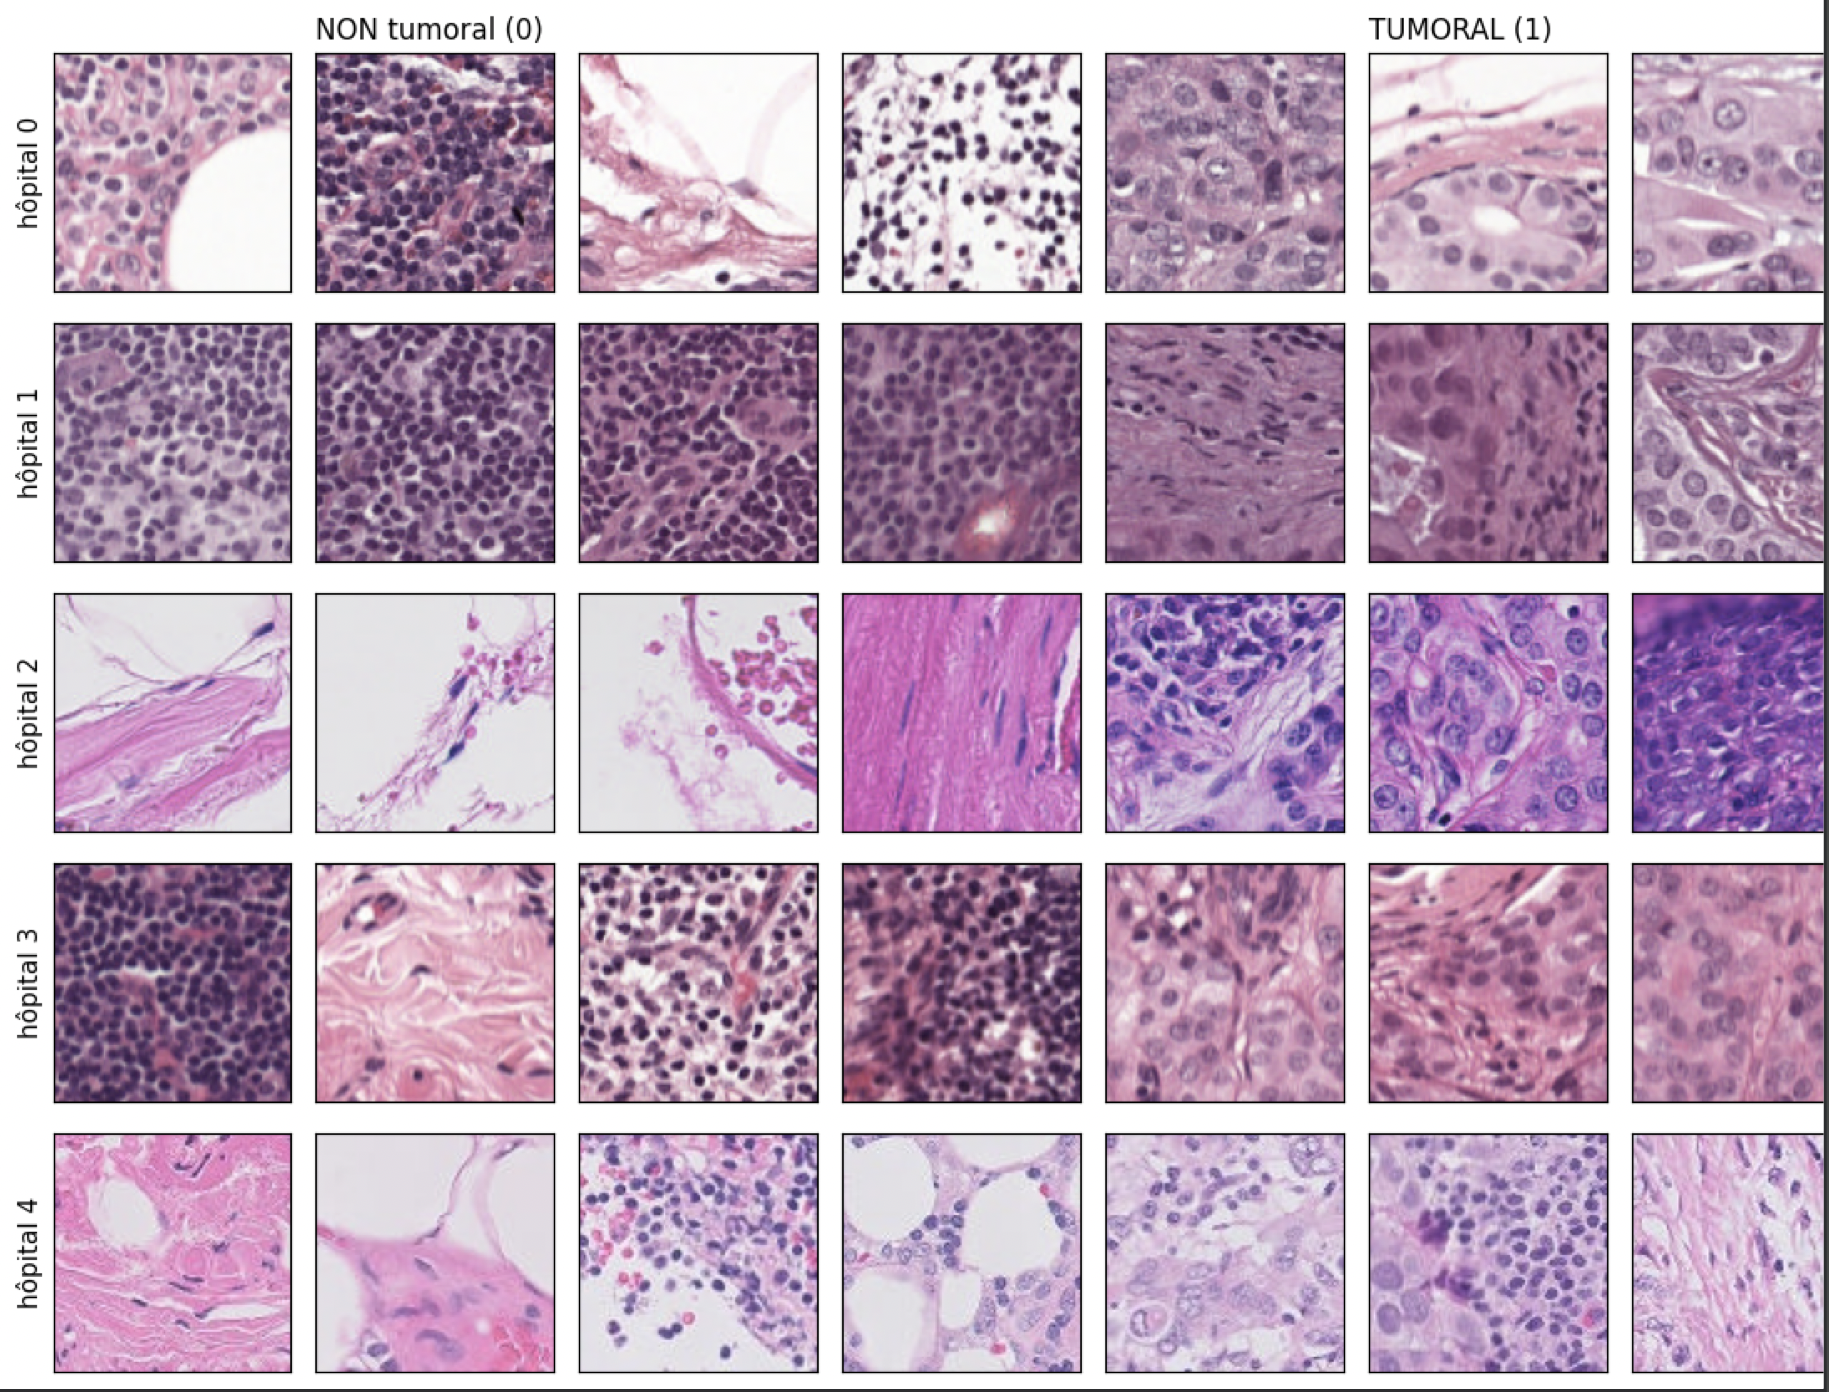
\includegraphics[width=\textwidth]{patchs.png}
\caption{Exemples de patchs : une ligne par hôpital ; à gauche non tumoral (0), à droite tumoral (1).
(Figure exportée du Colab, coupée à droite par l'impression.)}
\end{figure}

\paragraph{Ce qu'on observe.}
\begin{itemize}
  \item \textbf{Non tumoral} : surtout des nappes de \emph{lymphocytes} (petits noyaux ronds, sombres et serrés),
        de la graisse (grands vides blancs) ou du tissu de soutien rose.
  \item \textbf{Tumoral} : des cellules plus grandes, aux noyaux volumineux, plus clairs et irréguliers,
        disposées de façon désorganisée.
  \item \textbf{La couleur change beaucoup d'un hôpital à l'autre, à classe égale} : l'hôpital 2 est nettement
        plus violet et saturé, l'hôpital 4 plus pâle. Un humain s'adapte ; un modèle, pas forcément.
\end{itemize}

\subsection{Mesurer le changement de domaine : la couleur suffit-elle à reconnaître l'hôpital ?}
\textbf{Idée.} On résume chaque patch par 6 nombres de couleur : moyennes de rouge, vert et bleu,
saturation, quantité d'hématoxyline et quantité d'éosine (obtenues par « déconvolution de couleur », qui
sépare l'image en ses deux colorants). Puis on demande à un modèle très simple, une
\textbf{régression logistique}, de deviner l'hôpital à partir de ces 6 nombres seulement.
Le hasard donnerait 20 \% (5 hôpitaux). On mesure le score par \emph{validation croisée à 5 plis}
(on entraîne sur 4/5 des patchs, on teste sur le 1/5 restant, 5 fois, et on fait la moyenne).

\begin{figure}[H]
\centering
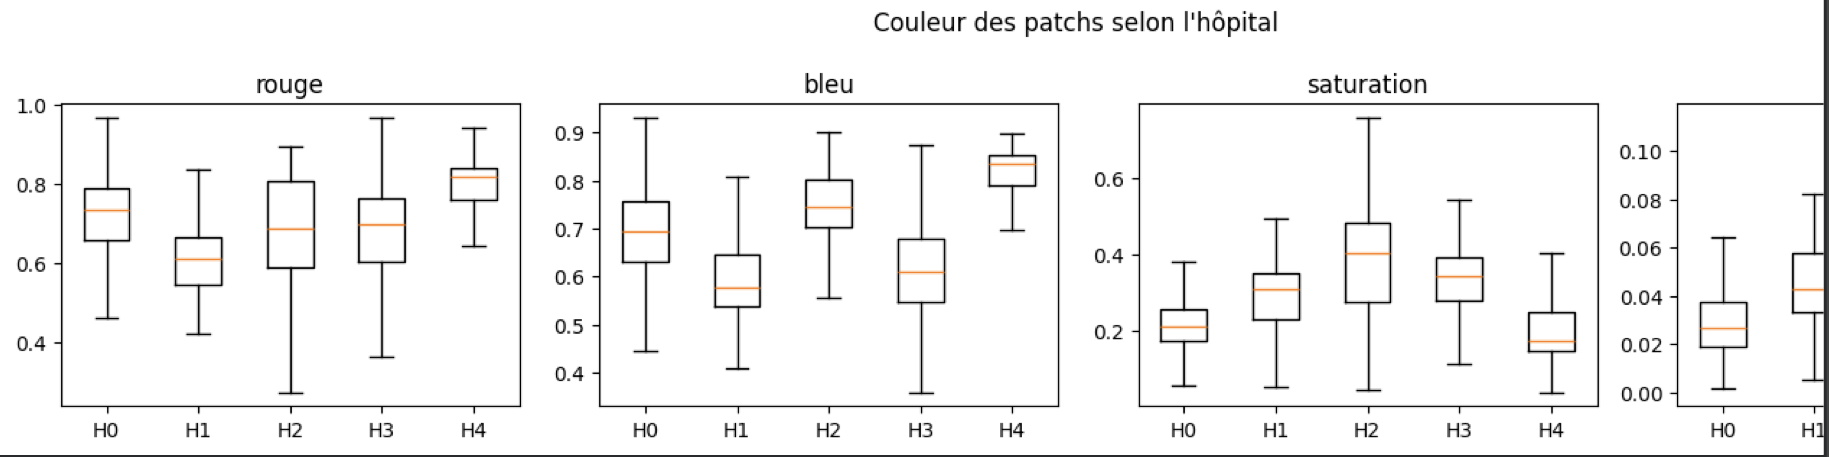
\includegraphics[width=\textwidth]{couleurs.png}
\caption{Distribution de la couleur des patchs selon l'hôpital (boîtes à moustaches : le trait orange est la
médiane, la boîte contient la moitié centrale des patchs).}
\end{figure}

\begin{constat}[Résultat : l'hôpital est reconnu dans 78 \% des cas avec 6 nombres de couleur]
Contre 20 \% pour le hasard. Les hôpitaux ont donc une \textbf{« signature » de couleur} très nette.
Danger : un CNN pourrait apprendre cette signature (« violet saturé = hôpital 2 ») au lieu de la
\emph{forme} des cellules. C'est pourquoi on évaluera toujours sur des \textbf{hôpitaux jamais vus}
pendant l'entraînement.
\end{constat}

\subsection{Les patchs d'une même lame sont-ils indépendants ?}
On affiche la position des patchs dans une lame, colorés par étiquette : les patchs tumoraux sont
\textbf{regroupés au même endroit} (la tumeur est une zone continue). Deux patchs voisins se ressemblent
énormément.

\begin{attention}[Conséquence : le risque de fuite de données]
Si on mélangeait les patchs au hasard entre entraînement et test, le modèle verrait au test des quasi-copies
d'images apprises : le score serait \textbf{artificiellement gonflé}. C'est une \textbf{fuite de données}
(\emph{data leakage}). D'où la règle de la partie suivante.
\end{attention}

%=====================================================================
\section{Découpage entraînement / validation / test, sans fuite}
%=====================================================================

\begin{resume}[Règle d'or]
On découpe \textbf{par patiente}, jamais par patch : toutes les images d'une patiente sont du même côté.
Un contrôle automatique dans le code (\texttt{assert}) vérifie qu'aucune patiente n'apparaît dans deux ensembles.
\end{resume}

\begin{table}[H]
\centering
\begin{tabularx}{\textwidth}{lXX}
\toprule
\textbf{Ensemble} & \textbf{Contenu} & \textbf{À quoi il sert} \\
\midrule
\texttt{train} & hôpitaux 0, 3, 4 — 80 \% des patientes & apprendre les poids du modèle \\
\texttt{val\_id} & hôpitaux 0, 3, 4 — les 20 \% autres patientes & choisir la meilleure époque et le seuil de décision \\
\texttt{val\_ood} & hôpital 1 (jamais vu) & vérifier la généralisation à un nouvel hôpital \\
\texttt{test\_ood} & hôpital 2 (jamais vu) & \textbf{test final}, regardé une seule fois à la fin \\
\bottomrule
\end{tabularx}
\caption{Les quatre ensembles. \emph{id} = \emph{in distribution} (mêmes hôpitaux que l'entraînement) ;
\emph{ood} = \emph{out of distribution} (hôpital inconnu).}
\end{table}

\begin{table}[H]
\centering
\begin{tabular}{lrrrr}
\toprule
\textbf{Ensemble} & \textbf{Non tumoraux} & \textbf{Tumoraux} & \textbf{Total} & \textbf{Patientes} \\
\midrule
\texttt{train} & 5\,349 & 6\,573 & 11\,922 & 21 \\
\texttt{val\_id} & 1\,506 & 630 & 2\,136 & 5 \\
\texttt{val\_ood} (hôpital 1) & 721 & 621 & 1\,342 & 8 \\
\texttt{test\_ood} (hôpital 2) & $\approx$ 1\,930 & $\approx$ 1\,925 & 3\,854 & 9 \\
\bottomrule
\end{tabular}
\caption{Effectifs obtenus (la ligne \texttt{test\_ood} était coupée dans l'export : valeurs déduites du
tableau par hôpital).}
\end{table}

\paragraph{Pourquoi deux validations ?} \texttt{val\_id} sert à \emph{régler} le modèle (époque, seuil) :
c'est ce qu'on ferait dans un vrai hôpital avec ses propres données. \texttt{val\_ood} sert à
\emph{surveiller} la généralisation pendant l'entraînement, sans toucher au test.

\paragraph{Pourquoi pas le découpage officiel de WILDS ?} WILDS propose un ensemble \texttt{id\_val} qui
reprend des patchs \textbf{des mêmes lames} que l'entraînement : c'est exactement la fuite décrite plus haut.
On a donc refait notre propre découpage par patiente.

\begin{oral}[Si la prof demande : « Pourquoi l'hôpital 2 en test ? »]
C'est le choix officiel du benchmark WILDS (hôpital 1 en validation hors domaine, hôpital 2 en test). C'est
aussi l'hôpital le plus différent en couleur (le plus violet), donc le test le plus exigeant. Et le suivre
permet de comparer nos chiffres à ceux publiés.
\end{oral}

%=====================================================================
\section{Le modèle : un CNN classique}
%=====================================================================

\subsection{Pourquoi un CNN ?}
Un \textbf{réseau de neurones convolutif} (CNN, \emph{convolutional neural network}) est conçu pour les
images. Au lieu de regarder chaque pixel séparément, il fait glisser de petits \textbf{filtres} (3 × 3 pixels)
sur l'image. Chaque filtre apprend à détecter un motif local : un bord, une texture ; puis, en empilant les
couches, des formes de plus en plus complexes (un noyau, un amas de cellules). Les mêmes filtres sont appliqués
partout dans l'image : un noyau tumoral est reconnu où qu'il soit.

\subsection{Les briques, une par une}
\begin{table}[H]
\centering
\begin{tabularx}{\textwidth}{lX}
\toprule
\textbf{Brique} & \textbf{Rôle} \\
\midrule
Convolution 3 × 3 & fait glisser des filtres dont les valeurs sont apprises ; produit des « cartes de
caractéristiques » (une par filtre) \\
Normalisation de lot (BatchNorm) & recentre et réduit les valeurs à chaque couche : entraînement plus stable
et plus rapide \\
ReLU : $\max(0, x)$ & non-linéarité : sans elle, empiler des couches reviendrait à une seule opération
linéaire, incapable d'apprendre des formes complexes \\
Max-pooling 2 × 2 & garde le maximum de chaque carré 2 × 2 : divise la taille par 2 et rend le modèle tolérant
aux petits décalages \\
Pooling global & moyenne de chaque carte sur toute l'image : un seul nombre par filtre \\
Dropout (30 \%) & éteint au hasard 30 \% des neurones pendant l'entraînement : limite le sur-apprentissage
(le modèle ne peut pas compter sur un seul neurone) \\
Couche linéaire & combine les caractéristiques en 2 scores (\emph{logits}) : non tumoral / tumoral \\
\bottomrule
\end{tabularx}
\caption{Les briques du CNN.}
\end{table}

\subsection{L'architecture du petit CNN (appris de zéro)}
\begin{figure}[H]
\centering
\begin{tikzpicture}[
  bloc/.style={draw=bleu,fill=bleuclair,rounded corners,minimum height=1.1cm,text width=2.25cm,align=center,font=\footnotesize},
  fl/.style={-{Latex[length=2mm]},thick,bleu}]
\node[bloc,fill=gris] (in) {Image\\3 × 96 × 96};
\node[bloc,right=0.35cm of in] (b1) {Bloc 1\\32 filtres\\$\to$ 32 × 48 × 48};
\node[bloc,right=0.35cm of b1] (b2) {Bloc 2\\64 filtres\\$\to$ 64 × 24 × 24};
\node[bloc,right=0.35cm of b2] (b3) {Bloc 3\\128 filtres\\$\to$ 128 × 12 × 12};
\node[bloc,below=0.8cm of b3] (b4) {Bloc 4\\256 filtres\\$\to$ 256 × 6 × 6};
\node[bloc,left=0.35cm of b4] (gp) {Pooling global\\$\to$ 256 nombres};
\node[bloc,left=0.35cm of gp] (dr) {Dropout 0,3\\+ linéaire\\$\to$ 2 scores};
\node[bloc,fill=vertclair,draw=vert,left=0.35cm of dr] (out) {Softmax\\$\to$ $P(\text{tumoral})$};
\draw[fl] (in)--(b1); \draw[fl] (b1)--(b2); \draw[fl] (b2)--(b3); \draw[fl] (b3)--(b4);
\draw[fl] (b4)--(gp); \draw[fl] (gp)--(dr); \draw[fl] (dr)--(out);
\end{tikzpicture}
\caption{Chaque bloc = Convolution 3 × 3 $\to$ BatchNorm $\to$ ReLU $\to$ Max-pooling 2 × 2. La taille de
l'image est divisée par 2 à chaque bloc, le nombre de filtres est multiplié par 2.}
\end{figure}

\paragraph{D'où viennent les 389\,410 paramètres ?} Un paramètre est un nombre que le modèle ajuste pendant
l'entraînement. Une convolution 3 × 3 qui passe de $c_{\text{in}}$ à $c_{\text{out}}$ canaux a
$3 \times 3 \times c_{\text{in}} \times c_{\text{out}}$ poids :
\begin{align*}
\text{convolutions} &: 9 \times (3\cdot32 + 32\cdot64 + 64\cdot128 + 128\cdot256) = 387\,936\\
\text{BatchNorm (2 par canal)} &: 2 \times (32+64+128+256) = 960\\
\text{couche linéaire} &: 256 \times 2 + 2 = 514\\
\text{total} &: 389\,410.
\end{align*}
C'est petit : un ResNet18 en a environ 11 millions, un modèle de fondation de pathologie 86 millions ou plus.

\paragraph{L'option ResNet18.} Avec \texttt{MODELE = 'resnet18'}, on utilise à la place un réseau
\emph{résiduel} de 18 couches, \textbf{pré-entraîné sur ImageNet} (1,2 million de photos ordinaires :
chats, voitures…). On remplace sa dernière couche (1\,000 classes) par une couche à 2 sorties, et on
ré-entraîne tout le réseau sur nos patchs : c'est le \textbf{\emph{fine-tuning}} (ajustement fin).
Avantage : il sait déjà reconnaître bords et textures, il apprend vite.

\begin{oral}[Si la prof demande : « Pourquoi ces choix d'architecture (32 filtres, 4 blocs…) ? »]
C'est l'architecture classique la plus simple (style VGG) : on double les filtres quand on divise la taille,
pour garder à peu près le même volume d'information. 4 blocs suffisent pour passer de 96 à 6 pixels. On n'a
pas cherché à optimiser ces nombres : ce CNN est une \textbf{base de référence} (\emph{baseline}), le but est
qu'il soit simple, rapide et compréhensible. L'optimisation viendra avec les modèles de chacun.
\end{oral}

%=====================================================================
\section{Fonction de perte, optimiseur et entraînement}
%=====================================================================

\subsection{Des scores aux probabilités : le softmax}
Le modèle sort 2 scores bruts $(z_0, z_1)$, qui peuvent valoir n'importe quoi. Le \textbf{softmax} les
transforme en probabilités positives qui somment à 1 :
\[
p_k = \frac{e^{z_k}}{e^{z_0} + e^{z_1}}, \qquad p_1 = P(\text{tumoral} \mid \text{image}).
\]
Exemple : $z_0 = 1$, $z_1 = 3$ donne $p_1 = e^3/(e^1+e^3) \approx 0{,}88$.

\subsection{La fonction de perte : l'entropie croisée}
La \textbf{fonction de perte} (\emph{loss}) mesure à quel point le modèle se trompe ; tout l'entraînement
consiste à la faire baisser. Pour une classification, on utilise l'\textbf{entropie croisée}
(\emph{cross-entropy}). Pour un patch de vraie classe $y \in \{0, 1\}$ :
\[
\ell = -\log p_y \quad\text{soit}\quad \ell = -\big[\, y \log p_1 + (1-y)\log(1-p_1) \,\big].
\]
Sur un lot de $N$ images, on prend la moyenne $\frac{1}{N}\sum_i \ell_i$.

\begin{table}[H]
\centering
\begin{tabular}{cccc}
\toprule
\textbf{Vraie classe} & \textbf{Probabilité donnée $p_1$} & \textbf{Perte} & \textbf{Lecture} \\
\midrule
tumoral & 0,9 & $-\log 0{,}9 \approx 0{,}11$ & juste et sûr : presque pas puni \\
tumoral & 0,5 & $-\log 0{,}5 \approx 0{,}69$ & hésite : puni moyennement \\
tumoral & 0,1 & $-\log 0{,}1 \approx 2{,}30$ & faux et sûr de lui : très puni \\
\bottomrule
\end{tabular}
\caption{Intuition de l'entropie croisée.}
\end{table}

Une erreur commise avec assurance coûte très cher : le modèle est poussé à être confiant quand il a raison et
prudent quand il hésite.

\paragraph{Pourquoi pas de pondération des classes ?} Ici les deux classes sont à peu près équilibrées.
Sinon, on pourrait donner plus de poids à la classe rare : $\ell = -w_y \log p_y$
(en PyTorch : \texttt{nn.CrossEntropyLoss(weight=...)}). Ce sera utile sur les lames entières.

\begin{oral}[Si la prof demande : « Pourquoi l'entropie croisée et pas l'erreur quadratique ? »]
L'entropie croisée correspond au maximum de vraisemblance pour une variable de Bernoulli (oui/non) : c'est la
perte « naturelle » quand le modèle sort une probabilité. Elle punit fortement les erreurs confiantes et
donne des gradients bien plus forts que l'erreur quadratique quand le modèle se trompe nettement, donc
l'apprentissage est plus rapide.
\end{oral}

\subsection{L'optimiseur : comment on ajuste les poids}
À chaque étape :
\begin{enumerate}
  \item on passe un \textbf{lot} (\emph{batch}) de 128 images dans le modèle (passe avant, \emph{forward}) ;
  \item on calcule la perte ;
  \item la \textbf{rétropropagation} (\emph{backward}) calcule le \emph{gradient} : dans quelle direction modifier
        chaque poids pour faire baisser la perte ;
  \item l'optimiseur \textbf{AdamW} fait un petit pas dans cette direction. Adam adapte la taille du pas à
        chaque poids ; le « W » (\emph{weight decay}, coefficient $10^{-4}$) tire légèrement les poids vers 0,
        ce qui limite le sur-apprentissage ;
  \item le \textbf{taux d'apprentissage} (la taille du pas) suit un calendrier \textbf{OneCycle} : il monte
        progressivement jusqu'à $10^{-3}$, puis redescend vers presque 0, ce qui stabilise la fin.
\end{enumerate}
Une \textbf{époque} = un passage sur toutes les images d'entraînement. Avec 11\,922 images et des lots de 128,
une époque fait $\lceil 11\,922 / 128 \rceil = 94$ mises à jour.

\begin{lstlisting}[language=Python]
for x, y in lots_du_train:              # 94 lots par epoque
    perte = perte_fn(modele(x), y)      # 1-2. forward + perte
    opt.zero_grad(); perte.backward()   # 3. gradients
    opt.step(); calendrier.step()       # 4-5. mise a jour des poids et du pas
\end{lstlisting}

\subsection{Augmentation de données}
Un tissu au microscope n'a ni « haut » ni « bas ». À chaque lot, on applique au hasard des \textbf{miroirs}
(horizontal, vertical) et des \textbf{rotations de 90°}, sans changer l'étiquette. Le modèle voit plus de
variété et apprend la forme des cellules plutôt que leur orientation. Ces transformations sont faites
directement sur le GPU (rapide).

\subsection{Normalisation des entrées}
Les pixels (0–255) sont ramenés entre 0 et 1, puis \textbf{centrés-réduits} canal par canal (on retranche la
moyenne, on divise par l'écart-type). Ces moyenne et écart-type sont calculés \textbf{sur l'entraînement
uniquement} : les calculer sur le test serait une (petite) fuite.

\subsection{Le choix de la meilleure époque}
Après chaque époque, on calcule l'AUC (voir partie 7) sur \texttt{val\_id} et sur l'hôpital 1. On garde les
poids de l'époque qui a la \textbf{meilleure AUC sur \texttt{val\_id}} (jamais sur l'hôpital 2, qui reste
caché jusqu'au bout).

\begin{figure}[H]
\centering
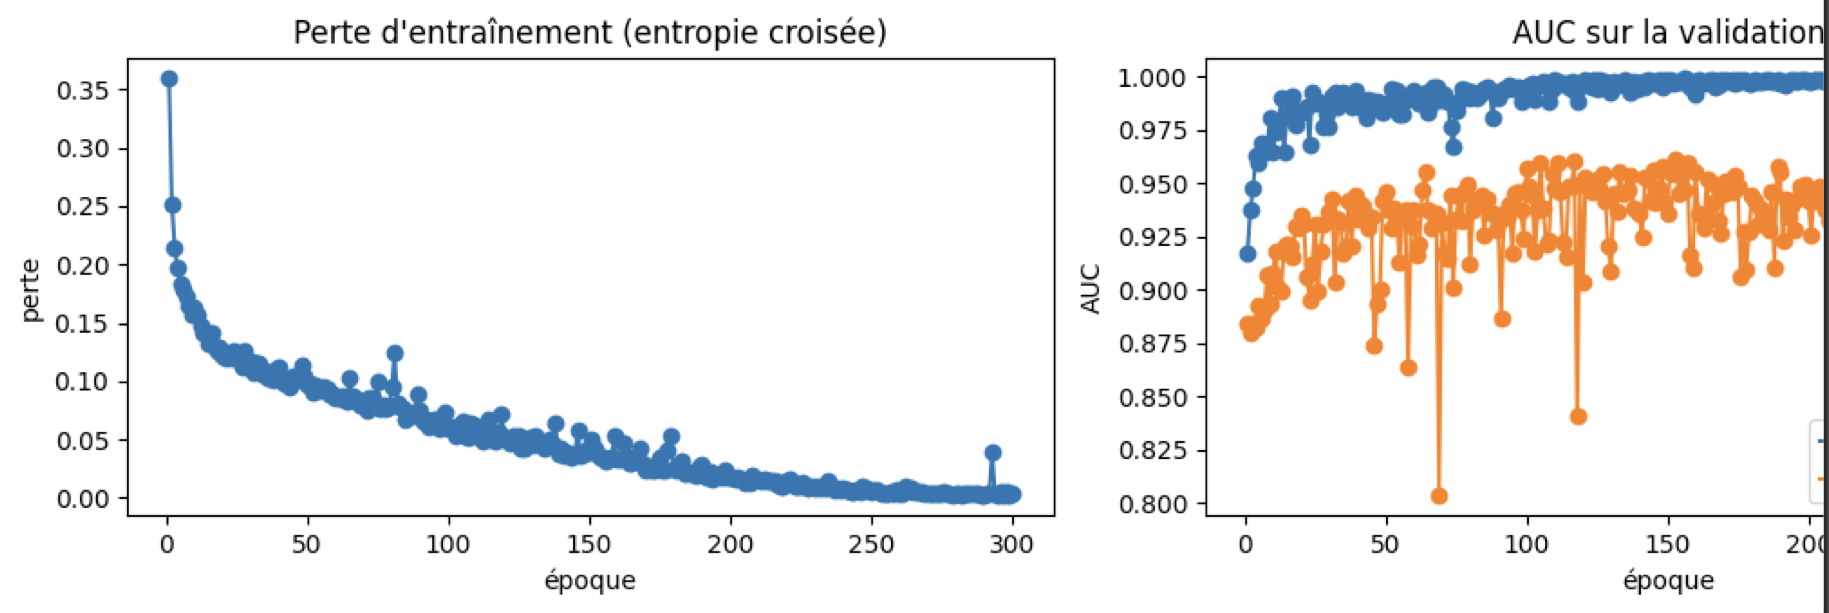
\includegraphics[width=\textwidth]{courbes.png}
\caption{Notre exécution à 300 époques. À gauche : la perte d'entraînement baisse régulièrement jusqu'à
presque 0. À droite : AUC sur \texttt{val\_id} (bleu) et sur l'hôpital 1 (orange). Époque retenue : 156.}
\end{figure}

\begin{constat}[Lecture des courbes]
\begin{itemize}
  \item La perte d'entraînement tombe de 0,36 à presque 0 : le modèle finit par connaître ses images
        d'entraînement \emph{par cœur}.
  \item L'AUC sur \texttt{val\_id} sature très vite autour de 0,995–0,999 : au-delà de quelques dizaines
        d'époques, elle ne bouge plus que dans les décimales (du bruit).
  \item L'AUC sur l'hôpital 1 plafonne vers 0,92–0,96 et fait des chutes brutales (jusqu'à 0,80) : le
        comportement hors domaine est \textbf{instable}.
  \item L'écart constant entre les deux courbes, c'est le \textbf{changement de domaine}.
\end{itemize}
\end{constat}

%=====================================================================
\section{Les métriques : définitions et à quoi elles servent}
%=====================================================================
Le modèle donne une probabilité $p_1$. Pour décider « tumoral / non tumoral », il faut un \textbf{seuil}
$s$ : on prédit « tumoral » si $p_1 \ge s$.

\subsection{La matrice de confusion}
\begin{table}[H]
\centering
\begin{tabular}{lcc}
\toprule
 & \textbf{prédit non tumoral} & \textbf{prédit tumoral} \\
\midrule
\textbf{vraiment non tumoral} & VN (vrai négatif) & FP (faux positif = fausse alerte) \\
\textbf{vraiment tumoral} & \cellcolor{orangeclair}FN (faux négatif = \textbf{tumeur ratée}) & VP (vrai positif) \\
\bottomrule
\end{tabular}
\caption{Les quatre cas possibles. La case orange est celle qu'on veut minimiser en priorité.}
\end{table}

\subsection{Les métriques}
\begin{table}[H]
\centering
\small
\begin{tabularx}{\textwidth}{l>{\centering\arraybackslash}p{3.4cm}X}
\toprule
\textbf{Métrique} & \textbf{Formule} & \textbf{Question à laquelle elle répond} \\
\midrule
Sensibilité (rappel) & $\dfrac{VP}{VP+FN}$ & Parmi les vraies tumeurs, combien sont trouvées ?
\textbf{Notre métrique prioritaire.} \\[8pt]
Spécificité & $\dfrac{VN}{VN+FP}$ & Parmi les tissus sains, combien sont bien reconnus comme sains ? \\[8pt]
Précision (VPP) & $\dfrac{VP}{VP+FP}$ & Quand le modèle dit « tumoral », a-t-il raison ? \\[8pt]
Exactitude (\emph{accuracy}) & $\dfrac{VP+VN}{\text{total}}$ & Part de bonnes réponses. Trompeuse si les classes
sont déséquilibrées (dire toujours « sain » sur une lame à 1 \% de tumeur donne 99 \%). \\[8pt]
F1 & $\dfrac{2\cdot\text{préc.}\cdot\text{sens.}}{\text{préc.}+\text{sens.}}$ & Compromis entre précision et sensibilité. \\[8pt]
AUC ROC & aire sous la courbe ROC & Probabilité qu'un patch tumoral pris au hasard reçoive un score plus élevé
qu'un patch sain pris au hasard. 0,5 = hasard, 1 = parfait. \textbf{Ne dépend pas du seuil.} \\[8pt]
AUC PR & aire sous la courbe précision–rappel & Idem, mais centrée sur la classe positive : plus informative
quand les tumeurs sont rares. \\
\bottomrule
\end{tabularx}
\caption{Les métriques utilisées.}
\end{table}

\paragraph{La courbe ROC.} On fait varier le seuil de 1 à 0. Pour chaque seuil, on place un point :
en abscisse le taux de fausses alertes ($1 - \text{spécificité}$), en ordonnée la sensibilité. Un bon modèle
monte très vite vers le coin en haut à gauche. L'AUC est l'aire sous cette courbe.

\subsection{Le choix du seuil}
Le seuil 0,5 n'a rien de spécial. Comme rater une tumeur est grave, on \textbf{fixe le seuil sur
\texttt{val\_id} pour détecter 95 \% des tumeurs}, puis on l'applique \textbf{tel quel} aux hôpitaux 1 et 2.
C'est le test le plus réaliste : dans un nouvel hôpital, on ne peut pas régler le seuil sur les patientes
qu'on est en train de diagnostiquer. Le seuil 0,5 est donné à côté pour comparaison.

\begin{oral}[Si la prof demande : « Pourquoi ne pas se contenter de l'AUC ? »]
Parce que l'AUC mesure si le modèle \emph{classe} bien les patchs les uns par rapport aux autres, pas s'il
prend la bonne \emph{décision} avec un seuil donné. On va voir qu'un modèle peut avoir une bonne AUC sur un
nouvel hôpital (0,907) et pourtant rater 65 \% des tumeurs au seuil réglé ailleurs. En clinique, c'est la
décision qui compte.
\end{oral}

%=====================================================================
\section{Résultats de notre exécution et interprétation}
%=====================================================================

\subsection{Les chiffres}
Seuil choisi sur \texttt{val\_id} pour 95 \% de sensibilité : \textbf{0,972}.

\begin{table}[H]
\centering
\begin{tabular}{lccccc}
\toprule
\textbf{Ensemble} & \textbf{AUC ROC} & \textbf{AUC PR} & \textbf{Seuil} & \textbf{Sensibilité} & \textbf{Spécificité} \\
\midrule
\texttt{val\_id} (H0, H3, H4) & 0,999 & 0,997 & 0,972 & 0,951 & 0,999 \\
\texttt{val\_ood} (hôpital 1) & 0,947 & 0,936 & 0,972 & 0,804 & 0,910 \\
\texttt{test\_ood} (hôpital 2) & 0,907 & 0,909 & 0,972 & \cellcolor{orangeclair}\textbf{0,349} & 0,993 \\
\bottomrule
\end{tabular}
\caption{Petit CNN, 300 époques (époque retenue : 156), seuil fixé sur \texttt{val\_id}.}
\end{table}

\begin{figure}[H]
\centering
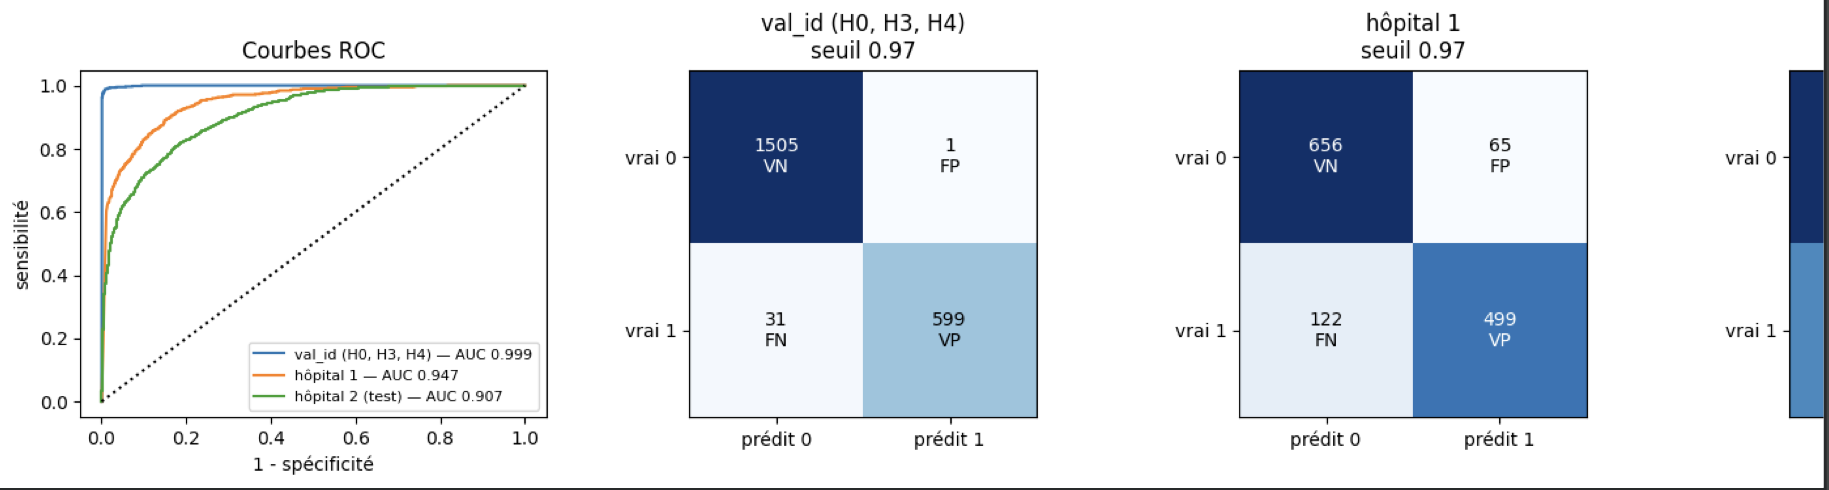
\includegraphics[width=\textwidth]{roc_confusion.png}
\caption{Courbes ROC des trois ensembles et matrices de confusion au seuil 0,97 (celle de l'hôpital 2 est
coupée par l'export).}
\end{figure}

\begin{table}[H]
\centering
\begin{tabular}{lcccc}
\toprule
\textbf{Ensemble} & \textbf{VN} & \textbf{FP} & \textbf{FN (tumeurs ratées)} & \textbf{VP} \\
\midrule
\texttt{val\_id} & 1\,505 & 1 & 31 & 599 \\
Hôpital 1 & 656 & 65 & 122 & 499 \\
Hôpital 2 & $\approx$ 1\,915 & $\approx$ 14 & $\approx$ 1\,250 & $\approx$ 670 \\
\bottomrule
\end{tabular}
\caption{Matrices de confusion au seuil 0,972 (hôpital 2 : valeurs approximatives reconstituées à partir de la
sensibilité et de la spécificité, la figure étant coupée).}
\end{table}

\subsection{Comment lire ces résultats}
\begin{enumerate}
  \item \textbf{L'AUC baisse dès qu'on change d'hôpital} : 0,999 $\to$ 0,947 $\to$ 0,907. C'est le
        changement de domaine mesuré en partie 3 : le modèle a appris en partie des couleurs propres à ses
        hôpitaux d'entraînement.
  \item \textbf{La sensibilité s'effondre au seuil fixé} : 95 \% visés, 80 \% sur l'hôpital 1, \textbf{35 \%}
        sur l'hôpital 2. Les probabilités sont décalées par la coloration : sur l'hôpital 2, beaucoup de vraies
        tumeurs reçoivent une probabilité inférieure à 0,972. \textbf{Un bon AUC ne garantit pas un modèle
        utilisable tel quel dans un nouvel hôpital.}
  \item \textbf{Le seuil est très haut (0,972)}, ce qui est un signal. Après 156 époques, le modèle est
        devenu extrêmement sûr de lui sur ses hôpitaux : presque toutes les tumeurs de \texttt{val\_id} ont
        $p_1 > 0{,}97$, donc le seuil « 95 \% de sensibilité » monte très haut. Sur un hôpital inconnu, où le
        modèle est moins confiant, ce seuil est beaucoup trop exigeant. Autrement dit : \textbf{entraîner plus
        longtemps a rendu le modèle plus confiant, pas plus robuste.}
  \item \textbf{Le choix de l'époque sur \texttt{val\_id} est fragile} quand l'AUC y est saturée à 0,998 : les
        époques ne se distinguent plus que par du bruit. L'époque 156 n'est pas meilleure qu'une époque 10 sur
        le plan hors domaine.
  \item \textbf{Prudence sur les décimales} : ces chiffres viennent d'un échantillon (19\,254 patchs, quelques
        patientes par hôpital). Ils varient d'une exécution à l'autre ; ce sont les \emph{tendances} qui
        comptent.
\end{enumerate}

\begin{attention}[Leçon pratique sur le nombre d'époques]
300 époques n'apportent rien par rapport à 8–10 : la perte d'entraînement continue de baisser (le modèle
apprend par cœur), mais l'AUC hors domaine plafonne dès les premières dizaines d'époques et le modèle devient
trop confiant. Pour comparer nos modèles entre nous, on recommande de rester autour de \textbf{10 époques pour
le petit CNN} et \textbf{3–4 pour un modèle pré-entraîné}. C'est aussi un très bon exemple de
\emph{sur-apprentissage au domaine} à montrer à l'oral.
\end{attention}

\subsection{Pour comparaison : nos résultats sur le jeu complet}
Avant le notebook, on avait entraîné plusieurs modèles sur les \textbf{455\,954 patchs} (sur Colab). Même
protocole : seuil fixé sur \texttt{val\_id} pour 95 \% de sensibilité, puis appliqué tel quel.

\begin{table}[H]
\centering
\small
\begin{tabular}{lcccc}
\toprule
\textbf{Modèle} & \textbf{AUC val\_id} & \textbf{AUC hôpital 1} & \textbf{AUC hôpital 2} & \textbf{Sensib. hôpital 2} \\
\midrule
Couleur + texture, régression logistique & 0,973 & 0,838 & 0,660 & 0,63 \\
Couleur + texture, forêt aléatoire & 0,965 & 0,901 & 0,896 & 0,99 \\
Petit CNN (5 époques) & 0,993 & 0,912 & 0,893 & 0,82 \\
ResNet18 pré-entraîné (3 époques) & 0,997 & \textbf{0,979} & \textbf{0,958} & 0,69 \\
\bottomrule
\end{tabular}
\caption{Jeu complet. Les deux premiers modèles n'utilisent pas d'images brutes mais des descripteurs calculés
à la main (statistiques de couleur et de texture).}
\end{table}

\begin{constat}[Le constat principal]
Le ResNet18 \emph{classe} le mieux (AUC 0,958 sur l'hôpital 2), mais au seuil appris ailleurs il
\textbf{rate 31 \% des tumeurs} de cet hôpital (13\,183 patchs sur 42\,527). Pour retrouver 95 \% de
sensibilité, il aurait fallu un seuil de 0,023 au lieu de 0,843. Le problème n'est pas la capacité à
reconnaître les tumeurs, \textbf{c'est le changement de domaine}. Notre exécution à 300 époques montre le
même phénomène, en plus marqué.
\end{constat}

\begin{oral}[Si la prof demande : « Comment comptez-vous corriger le changement de domaine ? »]
Trois familles de pistes, que l'équipe se répartit (partie 9) :
(1) \textbf{augmentation de couleur} pendant l'entraînement (on perturbe aléatoirement l'hématoxyline et
l'éosine, pour que le modèle ne puisse plus se fier à la couleur) ;
(2) \textbf{normalisation de coloration} (Macenko, Reinhard : on ramène toutes les images à une couleur de
référence avant le modèle) ;
(3) \textbf{modèles de fondation de pathologie} (Phikon, UNI), pré-entraînés sur des millions d'images de
tissus venant de nombreux hôpitaux, donc déjà habitués à la variété des colorations.
\end{oral}

%=====================================================================
\section{Pour la suite : chacun son modèle}
%=====================================================================
Ce notebook sert de \textbf{base commune} : mêmes données, même découpage par patiente, mêmes métriques, même
règle de seuil. Chacun teste une idée en modifiant seulement la partie 5 (le modèle) ou la partie 6
(l'entraînement), puis compare avec le tableau de la partie 7.

\paragraph{Pistes à se répartir.}
\begin{itemize}
  \item \textbf{Augmentation de couleur} (perturbation HED, \emph{color jitter}) ou \textbf{normalisation de
        coloration} (Macenko, Reinhard) : attaque directement le changement de domaine.
  \item \textbf{Autres CNN pré-entraînés} : ResNet50, EfficientNet, DenseNet (\texttt{torchvision.models}).
  \item \textbf{Modèles de fondation en pathologie} (Phikon, UNI…) : un réseau figé pré-entraîné sur des
        millions d'images de tissus, suivi d'une simple régression logistique.
  \item \textbf{Images agrandies} (96 $\to$ 224 pixels) pour les réseaux pré-entraînés sur ImageNet, qui ont
        été entraînés à cette taille.
  \item \textbf{Interprétabilité} : Grad-CAM, pour voir quelles zones du patch font décider le modèle (les
        noyaux ? ou juste la couleur de fond ?).
\end{itemize}

\begin{resume}[Règles communes pour que les comparaisons soient honnêtes]
\begin{enumerate}
  \item Ne jamais choisir un modèle, une époque ou un seuil en regardant l'hôpital 2.
  \item Toujours rapporter la \textbf{sensibilité au seuil fixé sur \texttt{val\_id}}, pas seulement l'AUC.
  \item Garder la même graine (\texttt{GRAINE = 0}), le même échantillon et le même découpage.
  \item Noter le nombre d'époques, la taille de lot et le temps de calcul.
\end{enumerate}
\end{resume}

%=====================================================================
\section{Les questions que la prof risque de nous poser}
%=====================================================================
Réponses courtes à connaître par cœur (les encadrés violets du document en donnent d'autres).

\begin{table}[H]
\centering
\small
\begin{tabularx}{\textwidth}{>{\raggedright\arraybackslash}p{5.3cm}X}
\toprule
\textbf{Question} & \textbf{Réponse} \\
\midrule
C'est quoi un patch ? & Un carré de 96 × 96 pixels découpé dans la lame, soit $\approx$ 0,1 mm de tissu. \\
C'est quoi l'étiquette exactement ? & 1 si le centre du patch est dans une zone tumorale dessinée par un
pathologiste. \\
Pourquoi découper par patiente ? & Les patchs voisins se ressemblent ; mélanger donnerait des quasi-copies
entre entraînement et test (fuite), donc un score gonflé. \\
Vos données sont-elles déséquilibrées ? & Non ici (50/50, choix de WILDS), mais oui en réalité (< 1 \% de
tumeur sur une lame). \\
Qu'est-ce que le changement de domaine ? & Le fait que les données de test (un nouvel hôpital) ne ressemblent
pas à celles d'entraînement (couleur différente). On l'a mesuré : l'hôpital se devine à 78 \% par la couleur. \\
Pourquoi l'entropie croisée ? & Perte standard quand le modèle sort une probabilité ; punit fortement les
erreurs confiantes. \\
C'est quoi une époque, un lot ? & Époque = un passage sur toutes les images d'entraînement ; lot = 128 images
traitées avant chaque correction des poids. \\
Pourquoi un seuil à 95 \% de sensibilité ? & Rater une tumeur est plus grave qu'une fausse alerte. \\
Pourquoi le régler sur \texttt{val\_id} ? & Dans un nouvel hôpital, on n'a pas les réponses pour régler le
seuil : c'est le cas réaliste. \\
Comment savoir que vous ne sur-apprenez pas ? & Validation séparée par patiente, test sur un hôpital jamais vu
et regardé une seule fois, dropout, weight decay, augmentation. \\
Pourquoi votre modèle est-il moins bon sur l'hôpital 2 ? & Couleurs différentes (plus violet) : les
probabilités sont décalées, le seuil réglé ailleurs ne convient plus. \\
Combien de temps ça tourne ? & $\approx$ 10 min de téléchargement, quelques secondes par époque sur GPU T4. \\
Votre résultat est-il stable ? & Sur l'échantillon, les décimales varient ; il faudra répéter avec plusieurs
graines. \\
\bottomrule
\end{tabularx}
\end{table}

%=====================================================================
\section{Questions à poser à la prof}
\label{sec:questions}
%=====================================================================
\noindent Même si certaines paraissent évidentes, mieux vaut les poser demain que de se tromper dans le
rapport. Elles portent surtout sur \textbf{ce qui vient après} ce notebook.

\subsection*{Sur le périmètre du projet}
\begin{enumerate}[label=\textbf{Q\arabic*.}]
  \item Est-ce que la classification de patchs (tumeur / pas tumeur) suffit, ou faut-il aller jusqu'au
        \textbf{stade pN de la patiente} (pN0, pN1mi, pN1, pN2) à partir des lames entières ?
  \item Est-ce qu'on peut travailler sur la version \textbf{WILDS} (patchs déjà découpés), ou faut-il partir
        des lames entières du challenge original ?
  \item Est-ce qu'un \textbf{échantillon} des données (comme dans le notebook) est acceptable pour les
        expériences, si on fait le résultat final sur le jeu complet ?
  \item Le jeu de test officiel de CAMELYON17 n'a pas de réponses publiques : est-ce que notre propre test
        (hôpital 2, jamais vu) est suffisant ?
\end{enumerate}

\subsection*{Sur les modèles}
\begin{enumerate}[label=\textbf{Q\arabic*.},resume]
  \item A-t-on le droit d'utiliser des \textbf{modèles pré-entraînés} (ResNet sur ImageNet, modèles de
        fondation de pathologie comme Phikon ou UNI), ou faut-il tout entraîner de zéro ?
  \item Si on utilise un gros modèle pré-entraîné (un \emph{Vision Transformer}, ou un \textbf{LLM /
        modèle multimodal}), doit-on \textbf{expliquer son architecture interne} en détail (attention,
        couches…), ou suffit-il d'expliquer comment on l'utilise ?
  \item Doit-on expliquer dans le rapport les \textbf{bases} (ce qu'est une convolution, la rétropropagation,
        l'entropie croisée), ou peut-on les supposer connues ?
  \item Chacun fait un modèle : faut-il à la fin \textbf{un seul modèle final} retenu, ou une
        \textbf{comparaison} de tous les modèles ? Combien de modèles au minimum ?
  \item Faut-il un modèle \textbf{classique} (non deep learning, ex. forêt aléatoire sur des descripteurs)
        comme point de comparaison ?
  \item Jusqu'où doit-on justifier les \textbf{hyperparamètres} (nombre d'époques, taille de lot, taux
        d'apprentissage) ? Faut-il une recherche systématique (grille), ou des choix argumentés suffisent ?
  \item Faut-il répéter les entraînements avec \textbf{plusieurs graines} et donner des intervalles de
        confiance, ou un seul run suffit ?
\end{enumerate}

\subsection*{Sur l'évaluation et les métriques}
\begin{enumerate}[label=\textbf{Q\arabic*.},resume]
  \item Quelle \textbf{métrique principale} attend-elle : AUC, sensibilité à seuil fixé, F1, ou (pour le stade)
        le kappa du challenge ?
  \item Notre choix de régler le seuil pour \textbf{95 \% de sensibilité} lui paraît-il pertinent, ou
        préfère-t-elle un autre critère ?
  \item Pour le \textbf{changement de domaine} : suffit-il de le \emph{mesurer}, ou attend-elle qu'on
        propose une \emph{correction} (normalisation de couleur, augmentation…) ?
\end{enumerate}

\subsection*{Sur l'interprétabilité et l'éthique (10 \% de la note)}
\begin{enumerate}[label=\textbf{Q\arabic*.},resume]
  \item Qu'attend-elle en \textbf{interprétabilité} : des cartes Grad-CAM sur quelques patchs, des cartes de
        chaleur sur les lames, autre chose ?
  \item Qu'attend-elle dans la partie \textbf{éthique} : biais entre hôpitaux, responsabilité en cas
        d'erreur, protection des données de santé (RGPD), place du médecin ? Quelle longueur ?
  \item Faut-il discuter du fait que les données viennent \textbf{uniquement des Pays-Bas} (généralisation à
        d'autres populations) ?
\end{enumerate}

\subsection*{Sur le rendu (rapport, code, oral)}
\begin{enumerate}[label=\textbf{Q\arabic*.},resume]
  \item Rapport de 15 pages : les \textbf{annexes}, la bibliographie et les figures comptent-elles dans les
        15 pages ? Format imposé (LaTeX, Word) ? Français ou anglais ?
  \item L'\textbf{exploration des données} (comme dans ce notebook) doit-elle être dans le corps du rapport ou
        en annexe ?
  \item Code : un \textbf{dépôt GitHub} suffit-il ? Doit-il être public ? Faut-il qu'il soit exécutable de bout
        en bout (avec un README) ?
  \item A-t-on le droit de \textbf{réutiliser du code} d'autres projets (GitHub, tutoriels) s'il est cité ?
  \item Doit-on \textbf{déclarer l'usage d'assistants IA} (ChatGPT, Claude…) pour le code ou la rédaction ?
        Sous quelle forme ?
  \item Oral de 10 minutes : \textbf{tout le monde doit-il parler} ? Une démo en direct est-elle souhaitée ou
        risquée ? Y a-t-il des questions après ?
  \item Comment est évaluée la \textbf{contribution individuelle} si chacun fait son modèle ?
  \item Y a-t-il un autre \textbf{point de suivi} avant le rendu du 27/11 ? Peut-on lui envoyer un brouillon ?
\end{enumerate}

%=====================================================================
\section{Glossaire}
\label{sec:glossaire}
%=====================================================================
\begin{description}[style=nextline,leftmargin=0.5cm,itemsep=1pt]
  \item[AUC] \emph{Area Under the Curve} : aire sous la courbe ROC ; 0,5 = hasard, 1 = parfait.
  \item[Augmentation de données] transformations aléatoires (miroir, rotation…) qui créent de la variété sans
        changer l'étiquette.
  \item[BatchNorm] normalisation des valeurs à l'intérieur du réseau, lot par lot.
  \item[Changement de domaine] différence entre les données d'entraînement et celles d'utilisation réelle (ici :
        la couleur selon l'hôpital).
  \item[CNN] réseau de neurones convolutif, spécialisé pour les images.
  \item[Dropout] extinction aléatoire de neurones pendant l'entraînement, contre le sur-apprentissage.
  \item[Entropie croisée] fonction de perte standard de la classification.
  \item[Époque] un passage complet sur toutes les images d'entraînement.
  \item[Fine-tuning] ré-entraîner un réseau pré-entraîné sur une nouvelle tâche.
  \item[Fuite de données] information du test qui « fuit » dans l'entraînement et gonfle les scores.
  \item[Gradient] direction dans laquelle modifier les poids pour faire baisser la perte.
  \item[H\&E] hématoxyline (noyaux, violet) et éosine (cytoplasme, rose).
  \item[ID / OOD] \emph{in distribution} (hôpitaux connus) / \emph{out of distribution} (hôpital inconnu).
  \item[Lame entière (WSI)] image numérisée complète d'une coupe de ganglion.
  \item[Logit] score brut du modèle avant le softmax.
  \item[Lot (batch)] groupe d'images traitées ensemble avant une mise à jour des poids.
  \item[Métastase] tumeur qui s'est propagée hors de son organe d'origine (ici, dans un ganglion).
  \item[Modèle de fondation] très gros réseau pré-entraîné sur des millions d'images, réutilisable pour
        beaucoup de tâches.
  \item[Paramètre / poids] nombre ajusté par le modèle pendant l'entraînement.
  \item[Patch] petit carré d'image (ici 96 × 96 pixels).
  \item[Seuil] valeur de probabilité au-dessus de laquelle on décide « tumoral ».
  \item[Sensibilité] part des vraies tumeurs détectées.
  \item[Softmax] fonction qui transforme des scores en probabilités.
  \item[Spécificité] part des tissus sains correctement reconnus.
  \item[Stade pN] classification de l'atteinte des ganglions (pN0 = aucune, pN1mi = micrométastase, etc.).
  \item[Sur-apprentissage] le modèle apprend ses données d'entraînement par cœur et généralise mal.
  \item[Taux d'apprentissage] taille des pas de correction des poids.
\end{description}

\section*{Références}
\begin{itemize}
  \item P. Bándi et al., « From detection of individual metastases to classification of lymph node status at the
        patient level: the CAMELYON17 challenge », \emph{IEEE Transactions on Medical Imaging}, 2019.
  \item P. W. Koh et al., « WILDS: A Benchmark of in-the-Wild Distribution Shifts », \emph{ICML}, 2021.
  \item K. He et al., « Deep Residual Learning for Image Recognition » (ResNet), \emph{CVPR}, 2016.
  \item I. Loshchilov, F. Hutter, « Decoupled Weight Decay Regularization » (AdamW), \emph{ICLR}, 2019.
  \item L. N. Smith, « Super-Convergence » (calendrier OneCycle), 2019.
  \item M. Macenko et al., « A method for normalizing histology slides for quantitative analysis », \emph{ISBI}, 2009.
\end{itemize}

\end{document}
